\documentclass[12pt, a4paper]{article}
\usepackage{graphicx}
\usepackage{fancyvrb}
\usepackage{listings}
\usepackage{epstopdf}
\usepackage{courier}
\usepackage{hyperref}
\usepackage{mathptmx}
\lstset {
basicstyle=\footnotesize\ttfamily,
showstringspaces=false,
numbers=left,
frame=single,
numbersep=5pt,
captionpos=b,
xleftmargin=17pt,
framexleftmargin=17pt,
framexrightmargin=5pt,
framexbottommargin=4pt,
stringstyle=\color{while}\ttfamily,
numberstyle=\tiny
}

\hypersetup{
 colorlinks=true,
 linkcolor=black,
 citecolor=black,
 urlcolor=blue,
}
\DefineVerbatimEnvironment{code}{Verbatim}{fontsize=\normalsize}{\fontfamily{pcr}}
\DefineVerbatimEnvironment{example}{Verbatim}{fontsize=\small}
\hyphenation{Ra-dix-IP-Look-up Pound-Rad-ix-IP-Look-up Bash-Rad-ix-IP-Look-up Read-Rad-ix-IP-Look-up}
\begin{document}
\author { 
Madhuri Venkatesh 
\\ UCLA 
\\ \textsl{madhuri@cs.ucla.edu}
\\
\\
\textsl{Supervised By:}
\\Eddie Kohler 
\\ UCLA/Harvard
\\ \textsl{kohler@cs.ucla.edu}
}
\title{Read Copy Update Framework for Userlevel Click}
\maketitle

\pagebreak
\section{Abstract}
High performance routing lookups are critically important for packet forwarding. With multi-core systems becoming more popular and more prevalent, leveraging them is key to improving performance. However, obtaining a correct, scalable and fast thread-safe solution remains challenging.\\

We have described an approach for providing thread-safety using \emph{Read Copy Update}. We have verified that we incur low read side overhead and that our approach performs up to 80\% better than reader-writer locks on read intensive workloads.
\section{Introduction}
The ever-increasing volume of network traffic over the internet demands highly efficient routing lookups. Link rates today exceed 40 Gbps, commodity network cards operate at over 15 Gbps but software routers struggle to comfortably scale beyond 10 Gbps. \\

Commodity machines with SMP multi-core architectures are growing in popularity. A software modular router such as Click running on commodity machines  can benefit greatly by exploiting parallelism on multi-core architectures.\\

Building a scalable and safe multi-core application is not a trivial task. Shared data structures in a multi-threaded application require synchronization for safe and correct access. Synchronization introduces overheads which attenuate the benefits of parallelism. Locks ultimately have the effect of  serialization such that only one thread accesses shared data at a time. A solution using locks also invariably involves the use of variables to synchronize access. These variables need to be accessed simultaneously by other processes or threads causing \emph{cache line bouncing}. This refers to the overhead of communicating the shared value across multiple caches which is very expensive. The larger the number of threads, the larger is the frequency of access of synchronization variables and the larger is the cost of synchronization. The lock based approach becomes less scalable and hence less attractive. \\

We wish to design a highly efficient multi-core solution. The typical workload is read intensive comprising of 90\% readers and less than 10\% updaters. \emph{Read Copy Update} \cite{readcopyupdate} scales efficiently on read intensive workloads and we seek to implement a Read Copy Update framework for the Click modular router. We compare the performance of our approach against a traditional lock-based approach using Click on a commodity machine. \\

The rest of the document is organized as follows. Section \ref{sec:background} gives the reader a background on the userlevel Click elements we are concerned with. Section \ref{sec:problem} describes why implementing a multicore solution was challenging. Section \ref{sec:solution} describes our solutions to the problem along with the implementation details. Sections \ref{sec:perfhypothesis} and \ref{sec:perfeval} describe the performance hypotheses and analysis.
\section{Related Work}
\emph{Routebricks} \cite{routebricks} proposes an architecture which enables higher packet processing speeds by distributing router functionality across multiple servers and multiple cores within a server. Their approach involves load balancing through Valiant Load Balancing (VLB). Their method of achieving faster packet processing is at a coarser level of granularity when compared to our approach.\\

Multiple efforts have been made at exploiting parallelism in the packet-flow mechanism in a software router. Wu and Wolf \cite{runtimepacketprocessing} have designed a run-time system which distributes the allocation of processing tasks to processor cores. It also balances the workload and maps the it across multiple cores. This parallelism is done at a task-level granularity.\\ 
%It does not look at synchronization of objects being used by the task. In our work we attempt to allow the task itself to be thread-safe so that it can be run on multiple cores.\\

Dobrescu et al. \cite{dobrescu} have proposed a technique in which the packet-processing flow and server characteristics are taken as input to formulate an optimization problem. A compiler would then solve this problem and output machine code which will optimize for throughput.
\section{Background}
\label{sec:background}
This section presents a brief overview of the \emph{RadixIPLookup} element. Our approach involved implementation and analysis using the RadixIPLookup element. We then extended our solution to other elements in Click. 
\subsection{An overview of RadixIPLookup}
The \emph{RadixIPLookup} element \cite{radixiplookup} is a class which is used to perform IP lookups. It uses a radix trie to perform the lookups and a vector to store the routes. This structure is explained in further detail. 
\subsubsection{The Radix Tree}
The radix tree is structured as a trie. The trie has  $2^8$ nodes at the first level, and $2^4$ nodes in the subsequent 6 levels. A lookup therefore has to traverse a maximum of 7 levels. This structure covers all $2^{32}$ IP addresses when the last level is fully occupied. Figure \ref{radixtree} shows the tree pictorially.\\
\begin{figure}[tph]
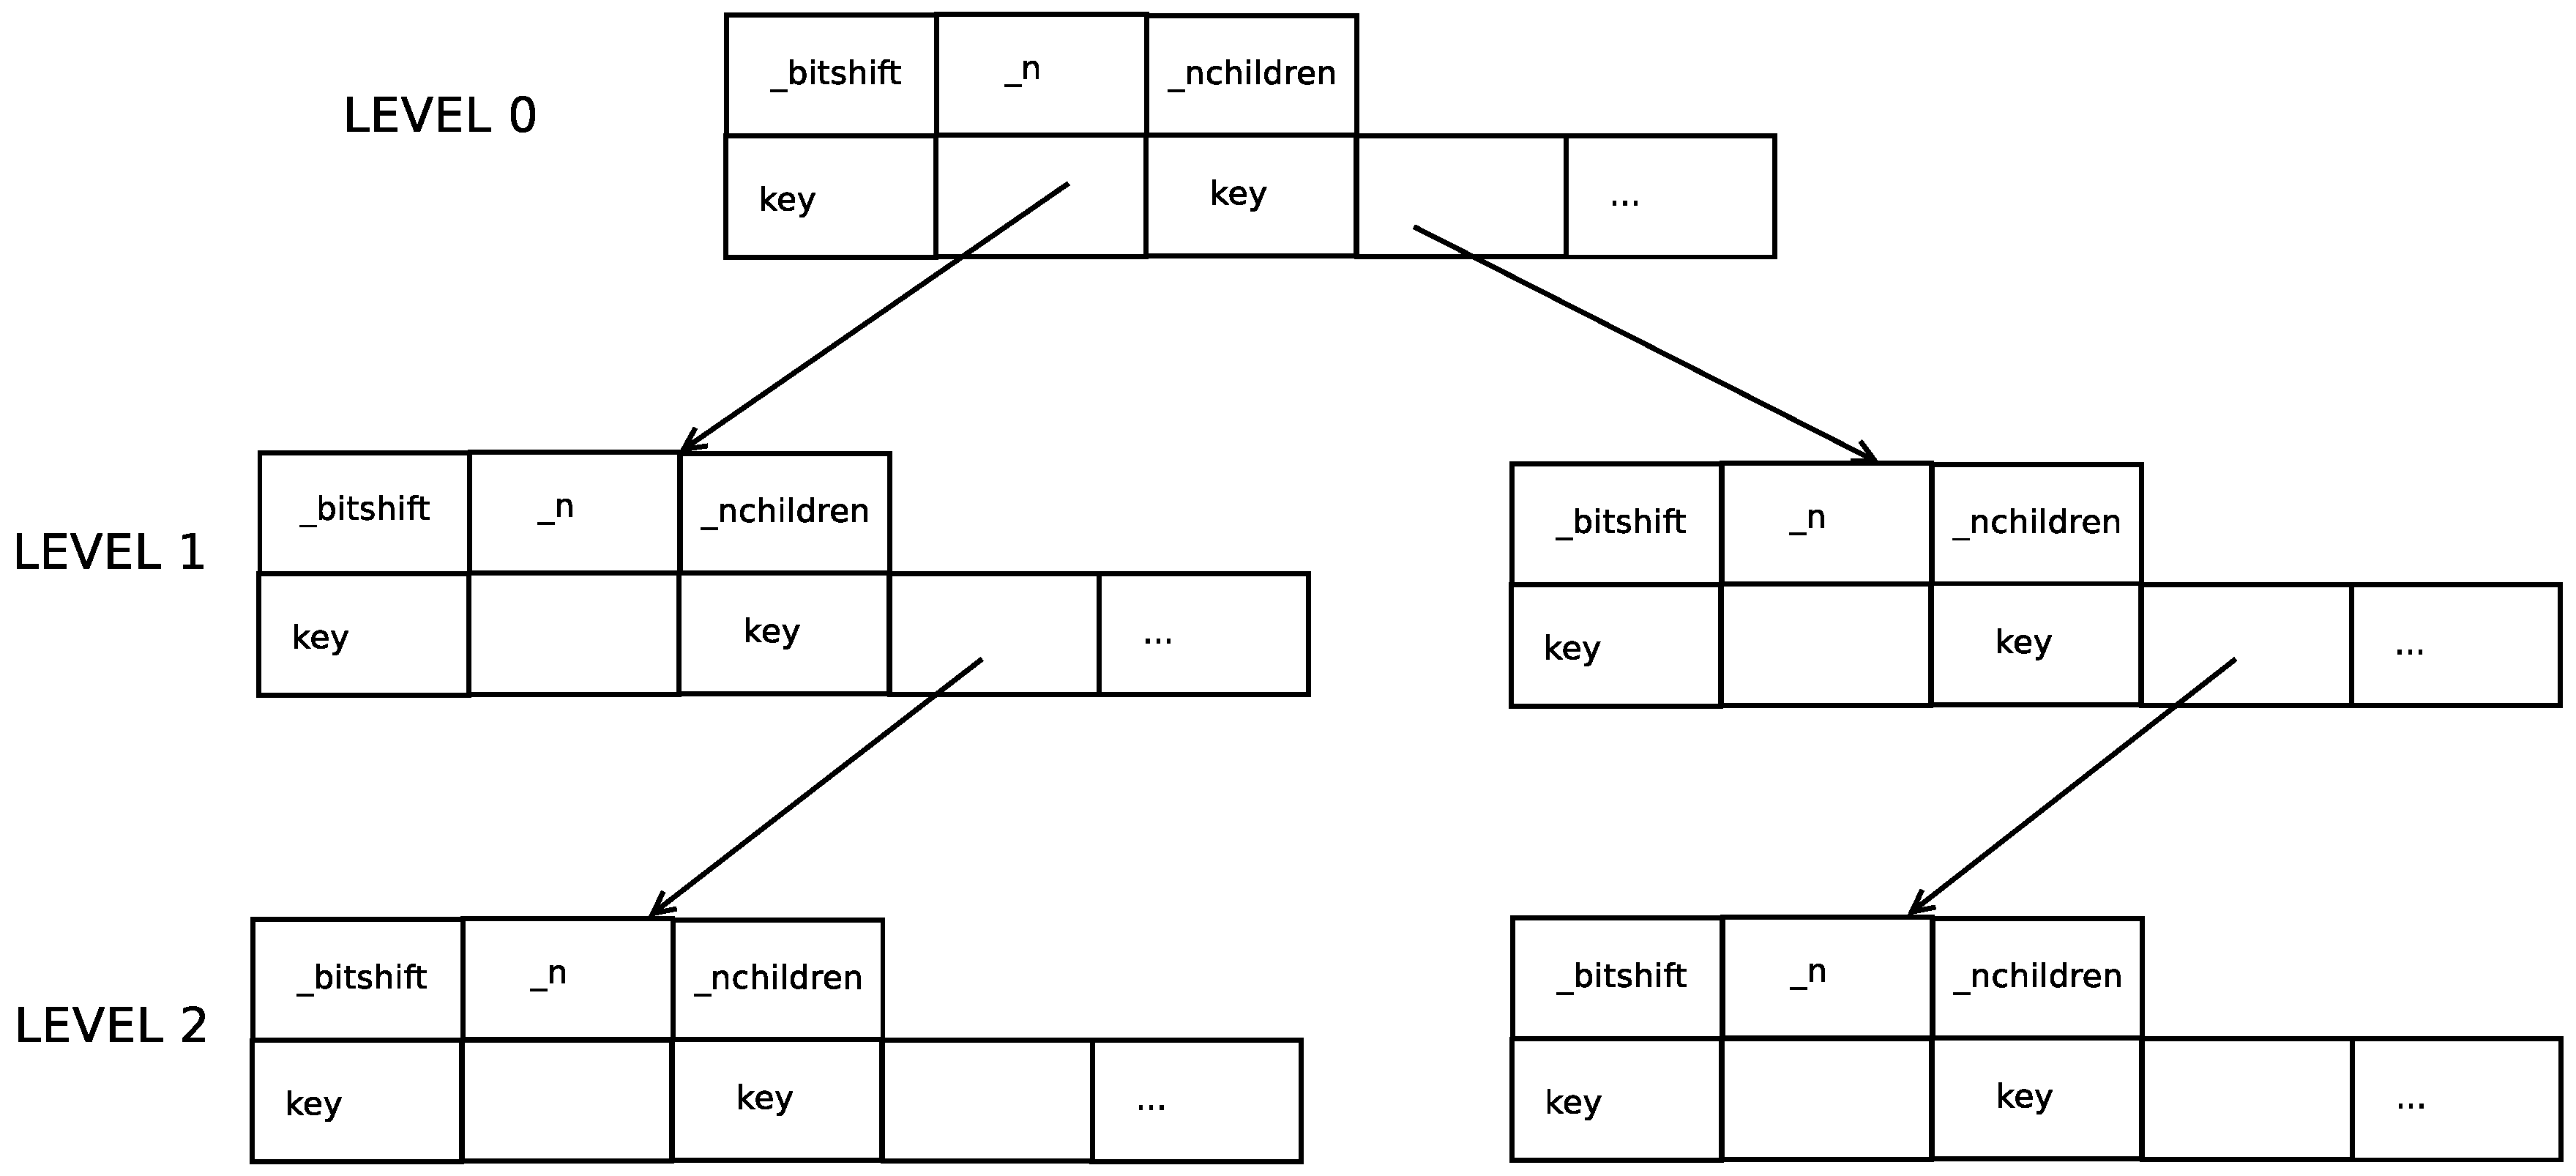
\includegraphics[scale = 0.2]{../images/diagrams/radixtree2.eps}
\caption{The Radix Tree}
\label{radixtree}
\end{figure}
\\Each level consists of radix nodes. The structure of the radix node is shown in Listing \ref{radixnode}. \emph{\_n} represents the number of radix nodes at that level. \emph{\_bitshift} represents the number of bits to be shifted at that level for prefix matching. For the radix node at level 0 \emph{\_n} is 256 and \emph{\_bitshift} is 24 (which is $32 - 8$). This means that the first 8 bits of the address are matched. For the radix nodes at level $1$, \emph{\_n} is 16 and \emph{\_bitshift} is 20 (which is $32 -8 -4$). This means that at level 1, the first 12 bits of the address have been matched.
\begin{lstlisting}[float=tph, caption = The Radix Class, label=radixnode]
class Radix {
  private:

    int _bitshift;
    int _n;
    int _nchildren;
    struct Child {
	int key;
	Radix *child;
    } _children[0];
...
...
}
\end{lstlisting}
The functions \emph{add\_route} and \emph{delete\_route} are used to add and delete routes into the routing table.
\paragraph{Lookups}
Routing Table Lookups for the Internet Protocol use a longest prefix match algorithm matching a candidate route with the highest subnet mask. The node at the top most level stores keys which need to match up to an 8 bit long prefix. The nodes in the next level store keys for routes which need to match up to a $12$ bit long prefix and so on. The last level stores keys which can match up to a $32$ bit long prefix. Listing \ref{lookup} shows the code for the lookup. Given an IP Address \emph{addr} which we need to lookup, we calculate the child pointer of the radix node which we need to follow using the \emph{bitshift} at that level. If the key for that child exists we repeat the process trying to obtain the longest prefix match. If it does not exist, we have found the longest prefix match for that node, so we return the key value. This key indexes into a vector which will return the gateway and port for the address.
\begin{lstlisting}[caption = The lookup function, label=lookup]
  static inline int lookup(const Radix *r, int cur, 
                           uint32_t addr) {
    while (r) {
      int i1 = (addr >> r->_bitshift) & (r->_n - 1);
      const Child &c = r->_children[i1];
      if (c.key)
      cur = c.key;
      r = c.child;
    }
    return cur;
  }
\end{lstlisting}
\subsubsection{The Vector class}
The Click library files provide an implementation of a generic Vector. A brief explanation of the use of the vector class in RadixIPLookup is described here. The RadixIPLookup element uses a vector of type IPRoute. IPRoute is a quintuple consisting of \emph{address}, \emph{mask}, \emph{gateway}, \emph{port} and \emph{extra}. The names of the first four fields are self-explanatory, Extra is used to recycle previously used but currently unused space within the vector. Extra is used to maintain a list of unused entries in the vector. We call this list the \emph{freelist}. If the index in the vector is in use Extra is set to $-1$, otherwise it stores the index of the next entry in the freelist. If an entry in the vector is deleted, the index of that entry is added to a free list.\\
\\The use of \emph{extra} is illustrated with the help of an example. Table \ref{tbl:vector} represents the vector at some point in time. The indices 2, 4 and 5 in the vector are currently being used (hence their \emph{\_vfree} is set to $-1$). The indices 0, 1 and 3 were in use earlier and have been deleted. They are part of the freelist. The \emph{\_vfree} points to the first entry in the freelist which will be used next. Briefly, \verb$freelist::{0 -> 3 -> 1,_vfree= 0}$. Let us say a new entry is added to the vector. So \emph{\_vfree} is reused, and the freelist is updated. Now, \verb$freelist::{ 3 -> 1, _vfree =3}$. Following another update, the index 3 will be used and the \verb$freelist::{1,_vfree=1}$. 
\\If the index 2 is now freed, \verb$freelist::{2 -> 1,_vfree = 2}$.
\\
\begin{table}
\begin{center}
\begin{tabular}{|l|l|l|l|l|l|}
\hline index & addr & mask & port & gw & extra \\ 
\hline 0 & 0.0.0.1 & 255.255.255.0 & 1& 22.34.198.3 & 3\\ 
\hline 1 & 1.1.0.1 & 255.255.255.0 & 1& 1.34.198.3 & -1\\
\hline 2 & 2.2.2.1 & 255.255.255.0 & 1& 2.34.198.3 & -1\\
\hline 3 & 1.0.0.1 & 255.255.255.0 & 1& 9.34.198.3 & 1\\
\hline 4 & 4.0.0.1 & 255.255.255.0 & 1& 8.34.198.3 & -1\\
\hline 5 & 4.0.0.1 & 255.255.255.0 & 1& 133.34.198.3 & -1\\
\hline
\end{tabular}
\end{center}
\label{tbl:vector}
\caption{Vector with routes}
\end{table}
\paragraph{Dynamic resize}
As is the case with most Vector classes, the Vector class in click has a \emph{push\_back()} function which adds an entry to the vector.
\\\\ If \_n exceeds \_capacity, a call to reserve\_and\_push\_back() is made. This dynamically increases the size of the vector. The code for push\_back() and reserve\_and\_push\_back() is given in Listing \ref{pushback} and Listing \ref{reserveandpushback}.

\section{The Problem}
\label{sec:problem}
Our goal is to improve lookup performance by allowing for multithread access to Click elements. In this section we look at existing problems which hinder safe multithreaded access.
\\\\The section is divided into unsafe access caused by multiple updaters (Updater-Updater Conflicts) and unsafe access caused by concurrent readers and updaters (Reader-Updater Conflicts). Concurrent updaters breed race conditions which might lead to an inconsistency in the data structures being used. A reader racing with an updater might read stale or invalid data.
\subsection{Updater-Updater Conflicts}
We now deal with race-conditions and conflicts arising due to multiple updaters running concurrently using the same instance of RadixIPLookup. When multiple threads use the same instance of RadixIPLookup, they access the same data structures within RadixIPLookup.
\paragraph{Radix Tree}
The radix tree suffers from Update-Update conflicts. If multiple updaters try to modify the same region of the tree, there is a race in \emph{change()} for the assignment of the child pointer. This could cause some of the updates to be lost and also cause a memory leak. The size of the memory leak can be equal to the depth of the tree times the size of a radix node.
\\\\The race described above is illustrated with the help of Listing \ref{change}.
\begin{lstlisting} [caption = Race in Change, label =change]
  int
  RadixIPLookup::Radix::change(uint32_t addr, uint32_t mask,
                                          int key, bool set)
  {
    int i1 = (addr >> _bitshift) & (_n - 1);
    // check if change only affects children
    if (mask & ((1U << _bitshift) - 1)) {
      if (!_children[i1].child
      && (_children[i1].child = make_radix(_bitshift - 4, 16)))
      ++_nchildren;
      if (_children[i1].child)
      return _children[i1].child->change(addr, mask, key, set);
      else
      return 0;
    }
    .......
    .......
    .......
  }
\end{lstlisting}
The change() code in Listing \ref{change} is used to create a radix node for a route with a specific address, and mask. The key passed as a parameter is the index into the vector where the route is stored. Looking at line number 9, we see that if there are multiple threads executing change(), there is a race for the assignment of the radix node. Multiple threads may call \emph{make\_radix()}, however only one pointer which is returned by \emph{make\_radix()} is assigned. This behavior can lead to memory leaks.
\paragraph{Vector}
When there are multiple updaters there is contention for acquiring an index into the vector. Many updaters trying to add a route might receive the same index value. If multiple updaters are given the same value of the index, there can be an inconsistency in the state of the vector. For example, the size of the vector might be stored wrongly or the freelist might be updated wrongly. Since the vector is resized dynamically, we could lose updates and have memory-leaks if reserve() is called concurrently.\\

We explain the conflicts mentioned above with examples using the \emph{add\_route()} function shown in  Listing \ref{addroute}.
\begin{lstlisting}[caption = The add\_route function, label=addroute]
  int
  RadixIPLookup::add_route(const IPRoute &route, 
                           bool set, 
                           IPRoute *old_route, 
                           ErrorHandler *)
  {
    int found = (_vfree < 0 ? _v.size() : _vfree), last_key;
    if (route.mask) {
      uint32_t addr = ntohl(route.addr.addr());
      uint32_t mask = ntohl(route.mask.addr());
      last_key = _radix->change(addr, mask, found + 1, set);
    } else {
      last_key = _default_key;
      if (!last_key || set)
      _default_key = found + 1;
    }
    if (last_key && old_route)
    *old_route = _v[last_key - 1];
    if (last_key && !set)
    return -EEXIST;
    if (found == _v.size())
    _v.push_back(route);
    else {
      _vfree = _v[found].extra;
      _v[found] = route;
    }
    _v[found].extra = -1;
    if (last_key) {
      _v[last_key - 1].extra = _vfree;
      _vfree = last_key - 1;
    }
    return 0;
  }
\end{lstlisting}
We consider two cases, one in which the concurrently executing threads retrieve an index from the freelist, the other in which the concurrently executing threads make a call to \emph{push\_back()} on the vector.

\paragraph{Case 1: Concurrent updaters use the freelist}
Assume the freelist is as follows before the execution of this code sequence:\\
\verb$freelist::{ 3 -> 1-> 5, _vfree =3}$. Consider the following sequence of events:
\begin{enumerate}
\item Thread 1 calls \emph{add\_route(X,1,NULL,NULL), X.addr =A, Y.mask = M}. The first parameter is the route, the second parameter asks the function to use the route supplied even if a route previously existed for that IP Address. The third parameter \emph{old\_route} retrieves a preexisting route for that IP if it is not set to NULL. The fourth parameter is the error handler.
\item Thread 2 calls \emph{add\_route(Y,1,NULL,NULL) Y.addr = A, Y.mask =M} .
\item Updater 1 and Updater 2 execute line 4 concurrently and recieve the same value of \emph{found}. Let us assume that \emph{found} is some key within the vector and is not equal to \emph{\_v.size()}. Updater 1 executes line 7 first. This updates the key in the radix tree to be the value \emph{found} which is $3$ according to our example.
\item Updater 2 executes line 7. The value of the key is set to \emph{found} which is $3$ since the freelist has not changed.
\item Updater 1 executes the remaining code in add\_route() including line 27 which sets \emph{\_v[found].extra} to $-1$ (which means that the index is in use). After the Updater 1 has finished executing add\_route(), the freelist reads \verb$freelist::{ 1-> 5, _vfree =1}$.
\item Updater 2 executes the remaining code sequence. It executes line 24 which sets \emph{\_vfree} to \emph{\_v[found].extra}. \emph{\_V[found].extra} has been set to $-1$ by Updater 1. Thus \emph{\_vfree} is now $-1$. \\
The state of the freelist is now \verb$freelist::{ 1-> 5,_vfree = -1}$. The correct state is \verb$freelist::{ 1-> 5, _vfree = 1}$. If \emph{\_vfree} is $-1$, it means that there are no more free keys in the vector, which is not true. This sequence brings the vector into an inconsistent state.
\end{enumerate}
\paragraph{Case 2: Concurrent updaters call \emph{push\_back()}}
Now consider the case when \_v.push\_back() is executed concurrently. For this we will look at the Click code from vector.cc in Listing \ref{pushback}.
\begin{lstlisting}[caption = The push\_back function, label=pushback]
  template <class T> inline void
  Vector<T>::push_back(const T& x)
  {
    if (_n < _capacity) {
      new(velt(_n)) T(x);
      ++_n;
    } else
    reserve_and_push_back(RESERVE_GROW, &x);
  }
\end{lstlisting}
We first consider the case when there is enough space in the vector: the expression $\emph{\_n} < \emph{\_capacity}$ evaluates to true. Updater1 and Updater2 use the same value of \emph{\_n}. The updater which wins the race installs its key at position i, and the other update is lost. If the aforementioned expresssion evaluates to false, we can have a different race which could lead to memory leaks. It is better understood with the help of the \emph{reserve\_and\_push\_back()} function shown in Listing \ref{reserveandpushback}.
\begin{lstlisting}[caption= reserve\_and\_push\_back(), label =reserveandpushback]
  Vector<T>::reserve_and_push_back(size_type want, 
                                  const T *push_x)
  {
    if (want < 0)
    want = (_capacity > 0 ? _capacity * 2 : 4);
    if (want > _capacity) {
      T *new_l = (T *) CLICK_LALLOC(sizeof(T) * want);
      if (!new_l)
      return false;
      for (size_type i = 0; i < _n; i++) {
        new(velt(new_l, i)) T(_l[i]);
        _l[i].~T();
      }
      CLICK_LFREE(_l, sizeof(T) * _capacity);
      _l = new_l;
      _capacity = want;
    }
    if (unlikely(push_x))
    push_back(*push_x);
    return true;
  }
\end{lstlisting}
Assume that both Updater1 and Updater2 execute code concurrently and that each of them have a reference to a new array which they have created in line 7: \emph{new\_l}.
\\Some of these races could bring the vector to an inconsistent state or cause memory leaks. For example: If both the updaters call CLICK\_LFREE() in line 14, we could have a segmentation fault. The assignment of \emph{new\_l} in line 15 is also a race. This could lead to a memory leak: The size of the leak is equal to the size of \emph{new\_l}. The other consequence is that one update will be lost.
\paragraph{Verifying conflicts in Click}
An approach similar to the one described in the Reader-Updater Conflicts section was followed here. We created a Click elements called BashRadixIPLookup and PoundRadixIPLookup which repeatedly add and delete the same route having the same address but different values of the port. Both BashRadixIPLookup and PoundRadixIPLookup run concurrently on the same instance of RadixIPLookup. This concurrency is ensured by using the \emph{StaticThreadSched()} element in the script.
\begin{code}
  BashRadixIPLookup::repeat 10,000 times {
    add_route (A,X);
    delete_route (A,X);
  }
  PoundRadixIPLookup::repeat 10,000 times {
    add_route (B, Y);
    delete_route (B,Y);
  } 
\end{code}
The tests resulted in segmentation faults and assertion failures, which did not occur if locks were acquired during updates.
\subsection{Reader-Updater Conflicts}
The conflicts in the RadixIPLookup element occur primarily in two data structures: vector used to store the routes, and the radix-tree which stores a key indexing into the vector. The sections below describe the conflicts which occur in each of these data structures.
\paragraph{Radix Tree:}
This section describes some of the reader-updater conflicts which exist and why they are not a source for concern. We take a look at a race which might arise and explain why it is not a serious problem.
\\
\\We now look at deletion of nodes within a radix tree. All pointers to the radix node are freed during a clean up phase of RadixIPLookup before it is destroyed. When a route is removed, the radix node corresponding to the route is not freed immediately. Instead all the radix nodes in the tree are deleted together at the end. This takes place in the call to free\_radix(). free\_radix() is called on an instance of RadixIPLookup just before the instance is destroyed.
\\
We will now look at a race condition which can occur in the radix tree when a reader and an updater execute concurrently. Consider a case where we have a reader and an updater running concurrently. The updater deletes route X, the reader performs a lookup on the very route X.
\begin{figure}[tph]
\begin{center}
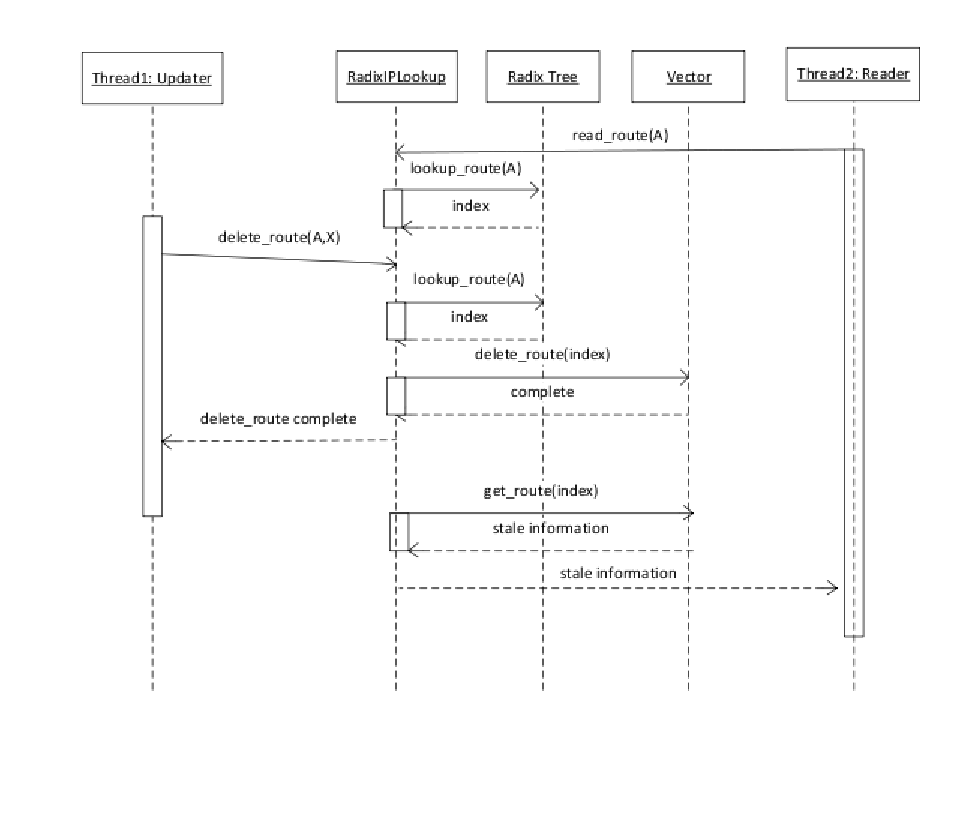
\includegraphics[scale=0.6]{../images/diagrams/race1eps.eps}
\end{center}
\caption{Race condition with a concurrent reader and updater}
\label{race1figure}
\end{figure}
\\\\
We have two threads one running: \emph{Updater:: \{remove Route X\}} and the other running: \emph{Reader::\{read Route A\}}. The reader might receive stale information for Route X. This happens if the reader acquires a reference to the radix node containing Route X before the pointer is removed from the tree (before the call to change(), line 24 in Listing \ref{removeroute}). The race is illustrated with the help of the sequence diagram in \ref{race1figure}. However, readers which execute after the updater has finished will not recieve stale data for Route X.
\begin{lstlisting}[caption= The remove\_route() function, label=removeroute]
  int
  RadixIPLookup::remove_route(const IPRoute& route, 
                              IPRoute* old_route, 
                              ErrorHandler*)
  {
    int last_key;
    if (route.mask) {
      uint32_t addr = ntohl(route.addr.addr());
      uint32_t mask = ntohl(route.mask.addr());
      // NB: this will never actually make changes
      last_key = _radix->change(addr, mask, 0, false);
    } else
    last_key = _default_key;
    if (last_key && old_route)
    *old_route = _v[last_key - 1];
    if (!last_key || !route.match(_v[last_key - 1]))
    return -ENOENT;
    _v[last_key - 1].extra = _vfree;
    _vfree = last_key - 1;
    if (route.mask) {
      uint32_t addr = ntohl(route.addr.addr());
      uint32_t mask = ntohl(route.mask.addr());
      (void) _radix->change(addr, mask, 0, true);
    } else
    _default_key = 0;
    return 0;
  }
\end{lstlisting}
The occurrence of the race mentioned above is rather rare: firstly a read intensive, infrequent update workload is expected but the aforementioned race is more likely in an update intensive workload. Secondly reads are fast compared to updates, so the possibility that a read operation starts before an update and ends after an update is quite small. That being said, we assume that the consequences of the race illustrated in the example above are acceptable. This is justified by the argument that the reader received a stale route: it was once valid route for the given address, and the ultimate price paid is the price of one wrong lookup.
\paragraph{Vector:}
The library files in Click include a generic dynamically resized Vector class. This class and its use in RadixIPLookup has been explained in the Background section. The conflicts are explained in the context of the add\_route() function which adds a route to the radix tree. The code for add\_route is given in Listing \ref{pseudoaddroute}. The way an index is obtained for insertion is summarized in the pseudocode below. 
\begin{lstlisting}[caption = Pseudocode for acquiring an index in add\_route, label=pseudoaddroute]
  if(free_list is not empty)
  {
    index = free_list;
    free_list = free_list -> next;
    _v[free_list.index] = val;
  }
  else 
  _v.push_back(val);
\end{lstlisting}
We can observe at least two inadmissible conflicts which can be caused by race conditions. Firstly, if two updaters and a reader run concurrently, the reader might get an index into an entry which has been freed and reused. The reader may end up receiving a route which is incorrect for the IP address in question. Secondly, a reader might access invalid memory in the presence of a concurrent updater. One must recall that the push\_back() operation dynamically resizes the vector if necessary. If an updater initiates a dynamic resize operation amidst a concurrent reader, the reader might access invalid memory occasioning a segmentation fault.

\paragraph{Verifying conflicts in Click}
The first conflict mentioned above was verified by running Click scripts. New elements were created and run in multi-threaded mode.The \emph{StaticThreadSched()} element was used to specify the thread on which the element must be run. Listing \ref{scriptlisting} facilitates a clearer picture of the use of \emph{StaticThreadSched()} for this case.
\begin{lstlisting}[caption = Click script for verifying reader-updater conflicts, label=scriptlisting]
Idle
 -> r :: RadixIPLookup106(
		0.0.0.0/0   8.1.1.1 0,
		) 
 -> Idle;

reader :: ReadRadixIPLookup106(r);
writer0:: BashRadixIPLookup106(r);
writer1 :: PoundRadixIPLookup106(r);

StaticThreadSched(
	reader 0,
	writer0 1,
	writer1  2);

DriverManager(stop);
\end{lstlisting}
We created a Click elements called BashRadixIPLookup and PoundRadixIPLookup which repeatedly add and delete a route having the for the same IP address but different port values.
\begin{code}
  BashRadixIPLookup::repeat 10,000 times {
    add_route (A,X);
    delete_route (A,X);
  }
  PoundRadixIPLookup::repeat 10,000 times {
    add_route (B, Y);
    delete_route (B,Y);
  } 
  ReadRadix:: repeat 10,000 times {
    port = Read (A);
  }
\end{code}
A and B are the addresses, X and Y are the values of the port. The least-common ancestor of A and B is the root node. The parameters for \emph{Add route} mentioned here are not the same as add\_route() used in \emph{RadixIPLookup}. The pseudocode presented above is simplified to illustrate the motive behind our method of verifying conflicts.
\begin{figure}[tph]
\fbox{
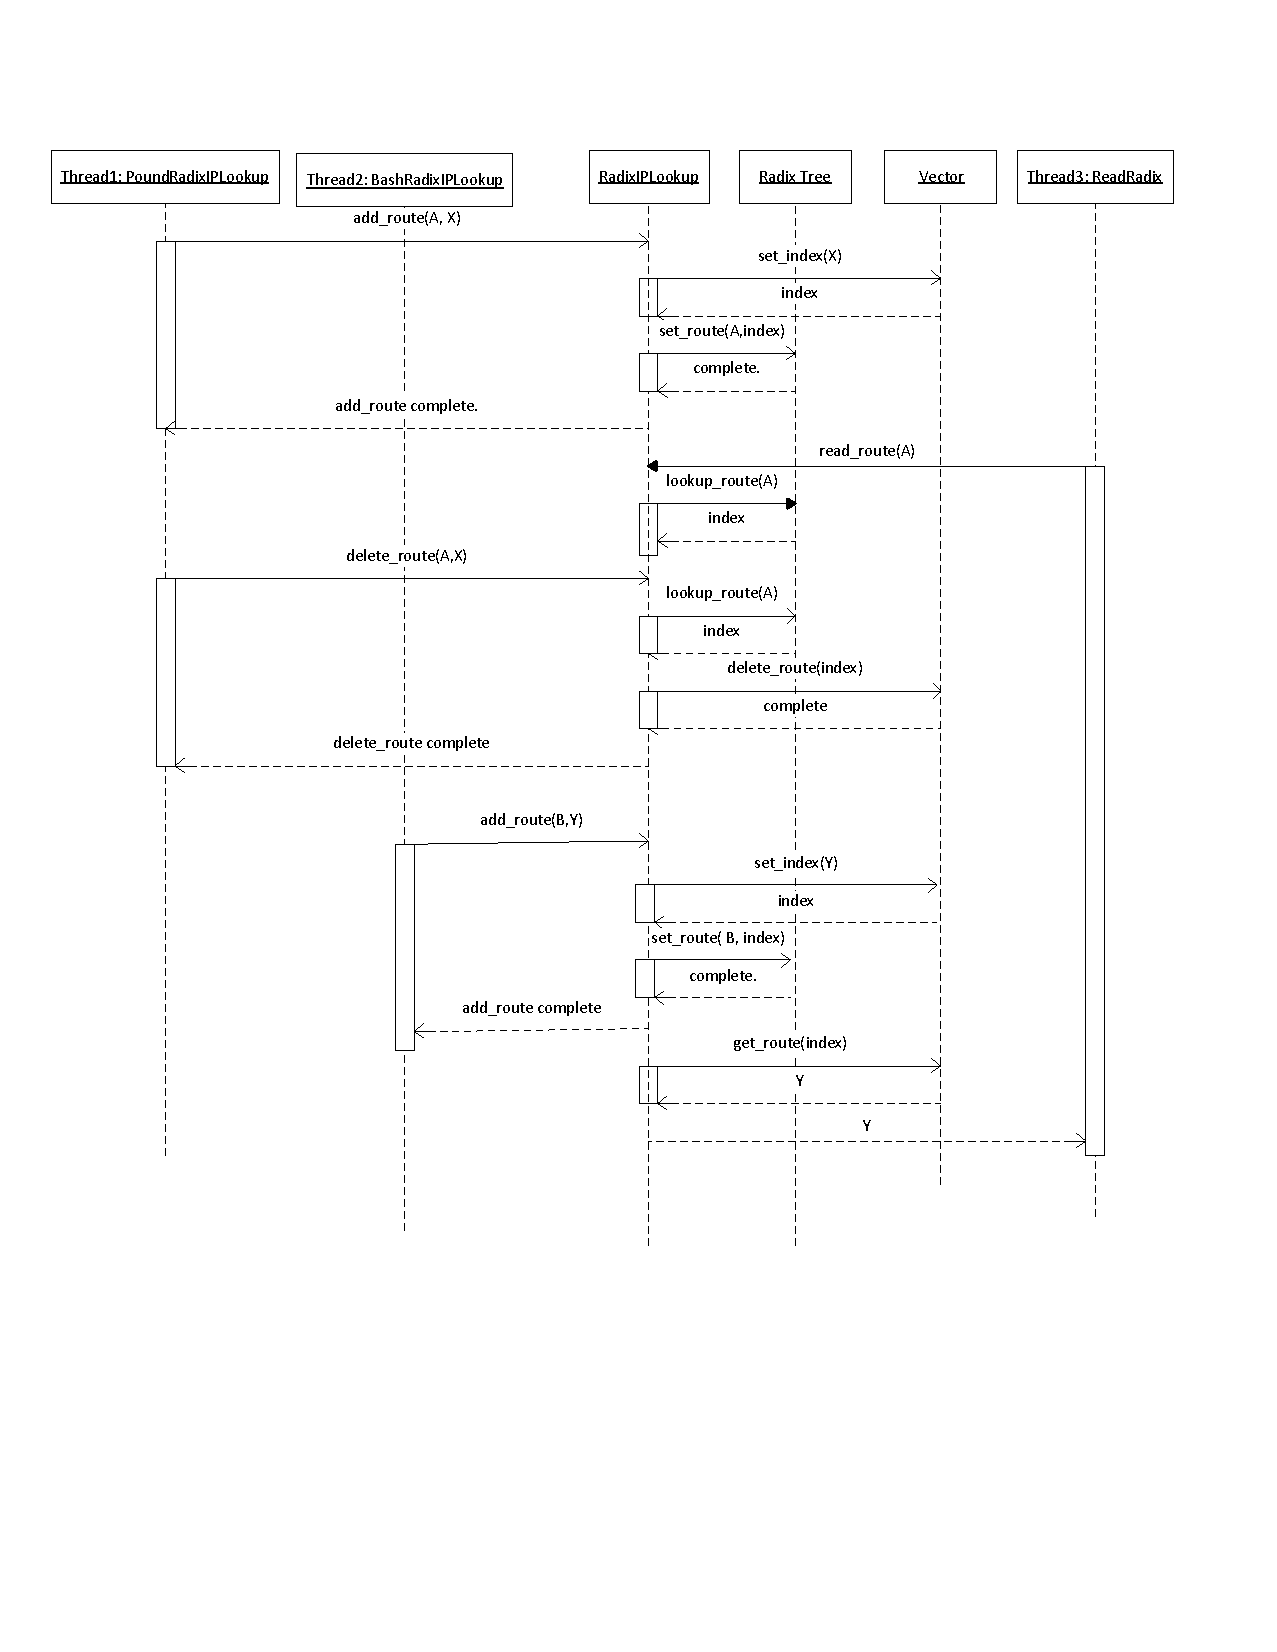
\includegraphics[scale=0.6]{../images/diagrams/race_reader.pdf}
}
\caption{Race condition with a concurrent reader and updater}
\label{race_readerfigure}
\end{figure}
\\
Locks are acquired during updates since we want to verify reader-updater conflicts as opposed to updater-updater conflicts. All three of these are run concurrently on the same instance of RadixIPLookup. The race is illustrated with the help of a sequence diagram in Figure \ref{race_readerfigure}.\\

A thread-safe implementation will have us expect that we always get X or the default route. A default route is returned if there was no prefix matching the route being looked up in the tree. But we see that the lookup sometimes returns Y which is incorrect.
\section{The Solution}
\label{sec:solution}
The race conditions described in the previous sections occur due to threads accessing shared data structures. In order to provide a thread-safe solution, several approaches were tried and their performance was compared. This section describes the different approaches tried in order to solve the problem. Coarse grained locking, fine-grained locking and Read Copy Update are the different methods we have tried. The Read Copy Update approach is the focus of this document, and a justification of its working and the implementation details are exposed in Section \ref{sec:rcu}.
\subsection{Coarse-grained locking}
Locking solves our problems since it prevents two threads from simultaneously accessing shared data. We chose a reader-writer lock, since the typical workload for a router is read intensive with few updates. In the absence of an updater, all readers can access shared data without contending for the lock.\\

The \emph{add\_route()} function using the reader-writer lock is shown in Listing \ref{addroutereaderwriterlocklisting}. A thread executing this function behaves as a writer since it updates shared data structures. A thread executing the \emph{lookup\_route()} function is a reader since it only reads shared data structures but does not modify them. The modified version of \emph{lookup\_route()} is shown in Listing \ref{lookuproutereaderwriterlocklisting}.
\begin{lstlisting}[caption = Reader-writer lock usage in lookup\_route(), label=lookuproutereaderwriterlocklisting,float=tph]
int RadixIPLookup107::lookup_route(IPAddress addr, 
                                   IPAddress &gw) const
{  
    _lock.acquire_read();
    int key = Radix::lookup(_radix, _default_key,
                             ntohl(addr.addr()));
    int port = -1;
    gw = 0;    
    if (key) {
	gw = _v[key - 1].gw;
	port =  _v[key - 1].port;
    }
    _lock.release_read();
    return port;
}
\end{lstlisting}

\begin{lstlisting}[caption = Reader-writer lock usage in add\_route(), label=addroutereaderwriterlocklisting,float=tph]
int
RadixIPLookup107::add_route(const IPRoute &route, 
                            bool set, 
                            IPRoute *old_route, 
                            ErrorHandler *)
{
  _lock.acquire_write();
  // ...
  // add_route() code
  // ...
  _lock.release_write();
  return 0;
}
\end{lstlisting}

\subsection{Fine-grained locking}
The reader-writer lock approach was improved with fine-grained locking in the updates. Every update in RadixIPLookup involves changes to the radix tree and changes to the underlying vector that it uses. These two changes are coupled together in the sense that one update depends on the outcome of the other. The code was restructured in add\_route() and remove\_route() in order to make fine grained locking possible.
\paragraph{Changes to add\_route}
The changes made to add\_route for fine grained locking are described.
add\_route is used to install a new route into the radix tree. This involves two steps:
\begin{enumerate}
\item Adding the route into the vector, and obtaining a key into the index where the new route is installed.
\item Updating the radix tree to reflect the key obtained in 1.
\end{enumerate}
The changes to the vector and changes to the radix tree are interdependent as seen in the \emph{add\_route()} function in Listing 5.
add\_route() was decoupled to use the following steps:
\begin{enumerate}
\item  Obtain an index to install the new route.
\item Update the radix tree with the key for the new route 
(creating new branches if necessary).
\item Update the freelist to reflect changes if it had been used in step 1.
\item Delete the old key in the vector if it was found for that route in step 2.
\end{enumerate}
After we have decoupled it in this way, we can create a thread safe implementation if each of the steps is atomic. The implementation involved locking and changes to the vector. The code for the modified version of add\_route can be found in Listing \ref{finegrainedaddroutelisting}.
\begin{lstlisting}[caption=Fine-grained add\_route(), label=finegrainedaddroutelisting,float=tph]
  int
  RadixIPLookup106::add_route(const IPRoute &route, 
                              bool set, 
                              IPRoute *old_route, 
                              ErrorHandler *)
  {
    int last_key;
    // we optimistically push back the route onto
    // the vector and don't do any free list management
    int found = insert_into_v(route);
    if (route.mask) {
      uint32_t addr = ntohl(route.addr.addr());
      uint32_t mask = ntohl(route.mask.addr());
      _rlock.acquire();
      last_key = _radix->change(addr, mask, found + 1, set);
      _rlock.release();
    } else {
      last_key = _default_key;
      if (!last_key || set)
      _default_key = found + 1;
    }
    if (last_key) { 
      if(old_route) { 
        _vlock.acquire();
        *old_route = _v[last_key - 1];
        _vlock.release();
      }
      if(set)
      remove_from_v(last_key);
      else {
        remove_from_v(found);
        return -EEXIST;
      }
    }
    return 0;
  }
\end{lstlisting}

\paragraph{Changes to remove\_route:}
The issues with \emph{add\_route()} also exist with \emph{remove\_route()}. This is because \emph{remove\_route()} also involves changes to the radix tree and changes to the underlying vector it uses in a similar manner. The restructured code for fine-grained locking works as shown below:
\begin{enumerate}
\item Search for the route in the radix tree and store it in last\_key.
\item If there was no route found, return with the appropriate error code.
\item If there was a route found, update the radix tree to reflect the change. 
\item Update the vector and its free-list.
\end{enumerate}
\paragraph{Changes to the Vector:}
The vector can be resized dynamically with a call to \emph{reserve()}. If multiple updaters concurrently call reserve(), there can be lost updates or segmentation faults due to the race conditions. Our goal was to modify the vector such that it is thread safe and wait-free for readers.\\

We created a two level vector: the first level has an array of pointers to other vectors and the second level stores the values. This introduces another level of indirection. An element whose index appears to be \emph{x} is actually located at \emph{\_v[pdx][idx]}, where \emph{pdx = x/BUCKETSIZE} and \emph{idx = x \% BUCKETSIZE}. This is illustrated in Figure \ref{bucketvector}. 
\begin{figure}[tph]
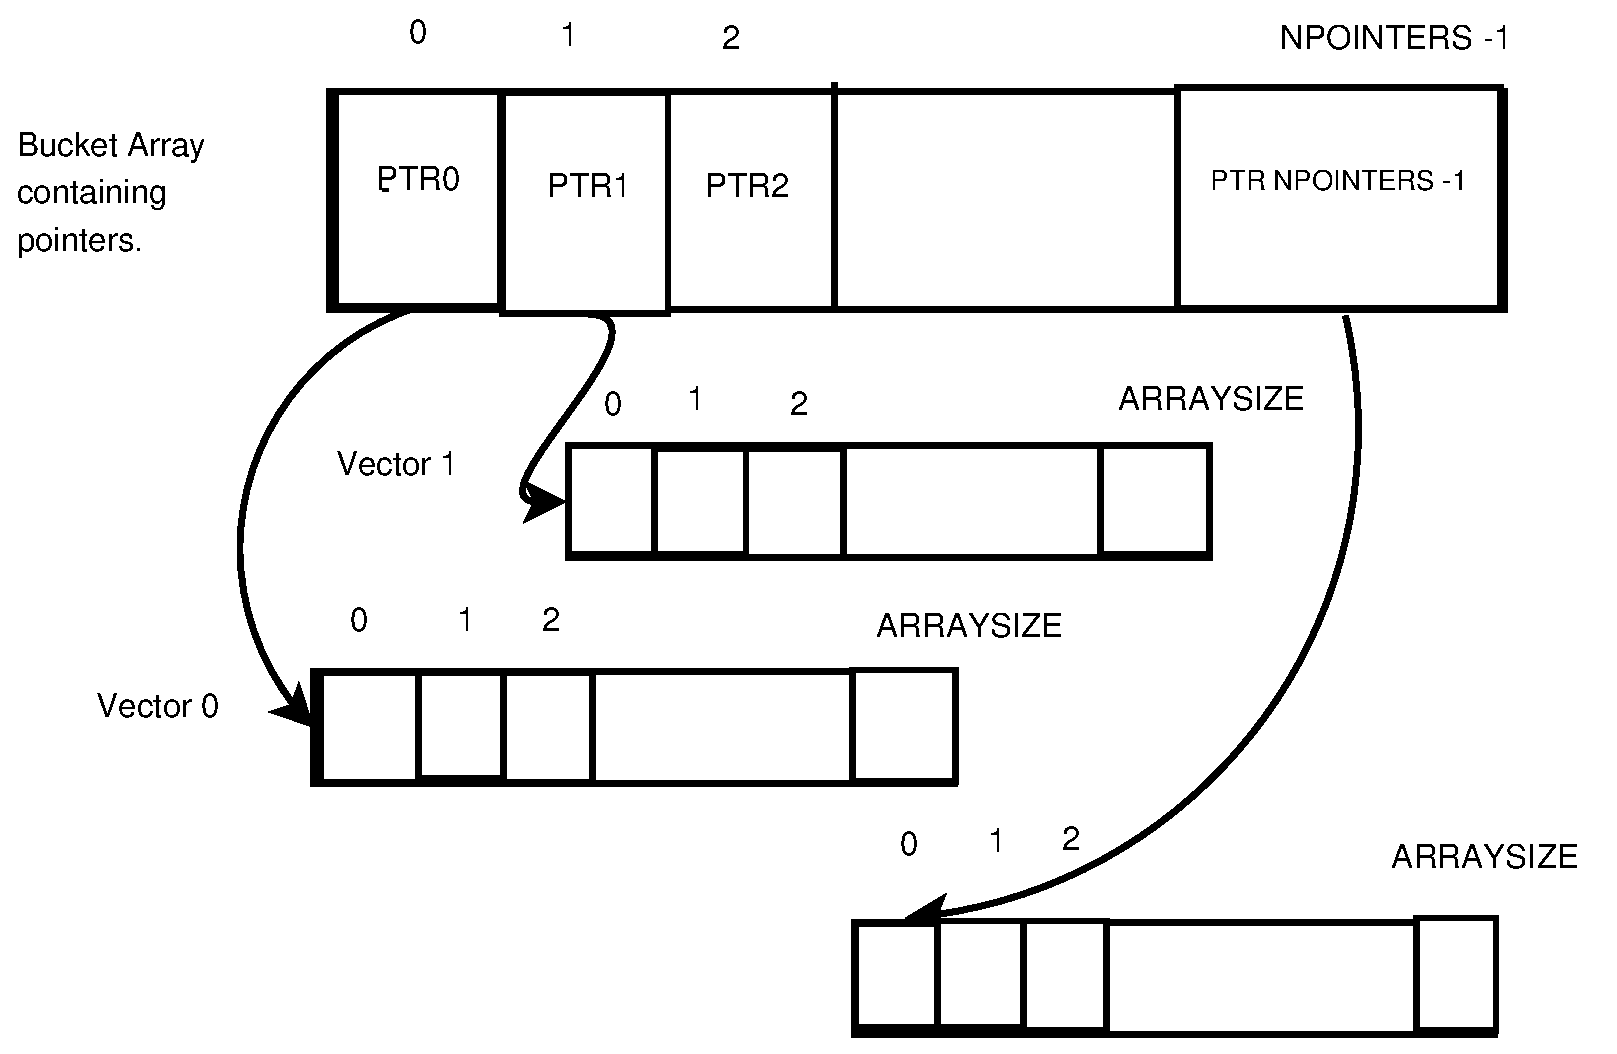
\includegraphics[scale = 0.4]{../images/diagrams/bucketvector.eps}
\label{bucketvector}
\caption{The bucket vector}
\end{figure}
Now, during a \emph{push\_back()} operation if there is enough space in the vector, the value will be added in one of the vectors. If there is no space, a new vector is created and a pointer to it is stored in the bucket array. This is safe for readers, since a reference acquired by a reader is always valid (assuming that the indices are not reused).\\

Since updaters can add new vectors to the bucket array, we still need to acquire a lock on updates. A lock is acquired in \emph{reserve()} in which the array is dynamically resized. This is done to prevent a race amongst concurrent updaters from executing \emph{push\_back()} in order to place new a vector into the bucket array. The code for \emph{reserve()} which includes this modification is shown in Listing \ref{bucketvectorreservelisting}.

We use compare-and-swap instructions to increment the \emph{\_capacity} variable in the vector. This ensures that \_capacity is incremented in an atomic manner by concurrent updaters.

\begin{lstlisting}[caption=Locking in reserve(), label=bucketvectorreservelisting]
template <class T> inline bool
BucketArray<T>::reserve() {
  _lock.acquire();
  if(_nelems >= capacity()) {
    T ** new_l = (T **) new unsigned char[\
      sizeof(T*) * (_npointers + 1)];
    if(!new_l) {
      _lock.release();
      return false;
    }
    
    new_l[_npointers] = (T *) CLICK_LALLOC(sizeof(T) 
                                          * ARRAY_SIZE);
    
    if(!new_l[_npointers]) {
      _lock.release();
      return false;
    }
    
    memcpy(new_l, _l, sizeof(T**) * _npointers);
    _reclaim_later.push_back((void*)_l);
    //_reclaimhook.schedule();

    _l = new_l;
    _npointers++;
    
  }
  _lock.release();
  return true;
}
\end{lstlisting}
\subsection{Using Read Copy Update in Click}
\label{sec:rcu}
Coarse and fine-grained locking solve the problems we have identified, but the locking system is still over 13 times slower in a pure reader workload consisting of four readers. Our goal is to develop a solution with no read-side overhead, so we turn to Read-Copy-Update \cite{readcopyupdate}.\\

Using RCU requires that we identify \emph{grace periods}: a state in which each thread has undergone at least one \emph{quiescent state}. A quiescent state is a state where a thread does not have any references to mutable data structures. This could be an idle-loop or a state where the thread is running code which does not access any shared data.\\

One of the main challenges in implementing RCU for Click was identifying quiescent states. One approach which works for RadixIPLookup  is using a timer expiry as a grace period. This approach was limited by the fact that it could not be arbitrarily extended to other Click elements. A more general approach involved using the Click scheduling loop. The next challenge was to provide an API which allows any userlevel element in Click to use RCU. 
\subsection{RCU using Timers}\label{sec:rcutimers}
\paragraph{Assumptions:}
The lookups on RadixIPLookup take place within 1000 ns. Thus it is somewhat safe to assume that a reader will finish one lookup within 500 ms.
We use this time-interval as a grace period or a quiescent state to free data-structures periodically.
\paragraph{Implementation:}
Click provides a Timer class which runs call-back functions at specified time-intervals. We use this to schedule a callback which reclaims freed data.
We maintain two lists: a \emph{reclaim\_now} list and a \emph{reclaim\_later} list. When an updater attempts to free an index we do not reclaim the index right away. Instead we add it to the reclaim\_later list.
In the timer callback function, we do the following:
\begin{enumerate}
\item Reclaim everything in the reclaim\_now list.
\item Swap the reclaim\_now list and the reclaim\_later list.
\end{enumerate}

RCU's main benefit is that we never block readers. This means that any mutable data structures being read must always be in a consistent state. The original vector was dynamically resized and there could be cases where there is allocated but uninitialized memory. To solve this problem, the modified version used the bucket array described earlier along with memory barriers. 
\subsection{RCU using Click Scheduling Loop}
The timer expiry as a quiescent state described in Subsection \ref{sec:rcutimers} works well for RadixIPLookup since each lookup is almost guaranteed to finish within 500 ms. This is not true of other elements in Click and it may not be possible to determine if and when a reader terminates. We wish to detect quiescent states for all other userlevel elements without having to know how long it takes for a reader task to complete. One approach is to use the scheduling loop in Click to detect quiescent states.
\paragraph{The Click RouterThread driver loop}
Click allows the user to supply the maximum number of threads it can use. Click has a class called \emph{RouterThread} which is responsible for running tasks scheduled by other Click elements. When Click is allowed to run with say $N$ threads, $N$ instances of \emph{RouterThread} are created. Each \emph{RouterThread} instance runs a \emph{driver()} function which runs tasks scheduled by Click elements in a loop. We will refer to this loop as the ``driver loop''. After running tasks, control periodically returns to the driver loop. A highly abridged version of the driver loop is shown in listing \ref{lst:driverloop}.
\begin{lstlisting}[caption = Pseudocode for the driver loop, label=lst:driverloop]
  void RouterThread::driver()
  {
    // initialization 
    driver_loop:
    run_tasks();
    // perform scheduling tasks etc
    // run timers
    // if driver has been stopped, exit the loop
    goto driver_loop;
  }
\end{lstlisting}
The instances of RouterThread are created by an instance of the Master class. Each thread is always in one of the following states:
\begin{itemize}
\item \emph{S\_PAUSED} : The thread is paused.
\item \emph{S\_BLOCKED} : The thread is blocked.
\item \emph{S\_TIMERWAIT} : The thread is waiting for a timer.
\item \emph{S\_RUNTASK} : The thread is running a task.
\item \emph{S\_RUNTIMER} : The thread is running a timer.
\end{itemize}
\paragraph{Local Epochs and the search for quiescent-states}
An epoch is the period during which the \emph{RouterThread} performs some activity: running timers, running tasks etc. Each instance of \emph{RouterThread} maintains an epoch number hereafter referred to as ``local epoch number''. The local epoch number is incremented every time control returns to the driver loop after finishing some activity. We also maintain a global epoch number. The global epoch number is incremented only when the local epoch numbers of all RouterThreads have been incremented. This is illustrated in the Figure \ref{rcufigure}. Every alternate global epoch we can free accumulated stale data. Specifically, we can safely free data accumulated by epoch $X$ in epoch $X+2$. Note that we cannot free stale data every time the global epoch number increases (i.e. at $X+1$) since a reader may still have a reference to some stale data. For example, in Figure \ref{rcufigure}, we cannot free all stale data accumulated in $GE=0$ during $GE=1$ since thread 3 might still have a reference to something which has been updated by Thread 2. The states which might be sharing references are highlighted using the same color.

\begin{figure}[tph]
\fbox{
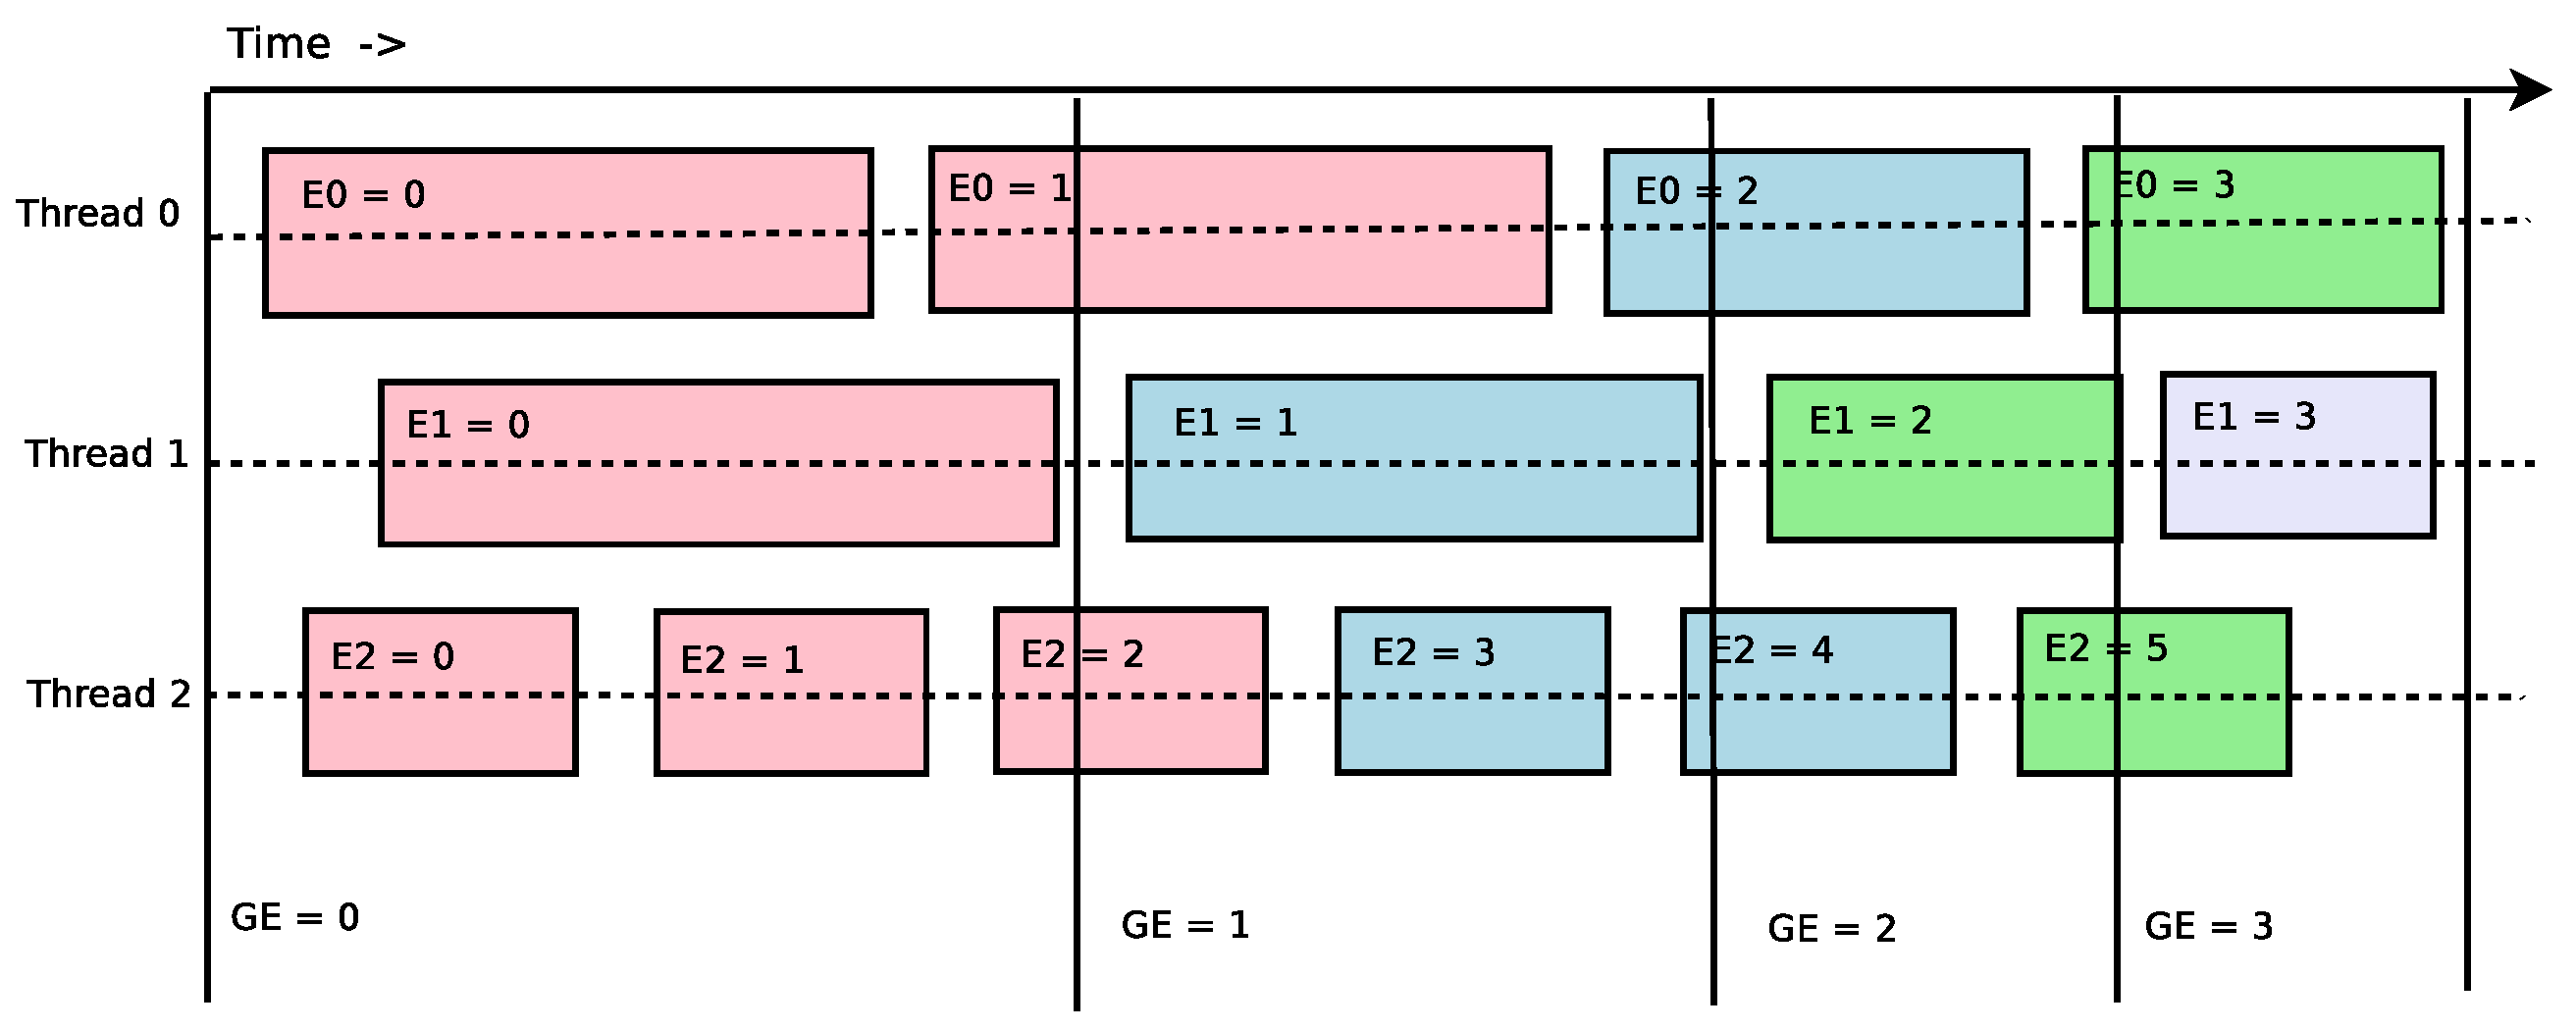
\includegraphics[scale=0.30]{../images/diagrams/rcu.eps}
}
\label{rcufigure}
\caption{Detecting quiescent states through global epochs}
\end{figure}

\paragraph{Implementation details}
In order to maintain epoch numbers we introduce a \emph{\_thread\_epoch} variable in the RouterThread class. The Master maintains the global epoch number. When control is returned to the driver loop after tasks are run, we increment the \_thread\_epoch variable and attempt to reclaim freed data. As in the Timer approach described earlier, we maintain two lists: a \emph{reclaim\_now list} and a \emph{reclaim\_later} list. An updater always adds any stale data to the relcaim\_later list. During a reclaimation, we free the data structures in the reclaim\_now list and swap the two lists. This ensures that we follow the freeing mechanism described in the above paragraph. Effectively, we can reclaim freed-data if every thread has changed its epoch variable since the last successful reclamation or if thread is blocked.
\subsection{Performance Hypothesis}
\label{sec:perfhypothesis}
RCU is known to work best for a reader-heavy workload with a small number of updaters. Our claim is that the RCU mechanism for click outlined above has almost zero reader-side overhead. Readers being lock-free and wait-free, we expect RCU performance to be comparable to the original version when there are only readers.\\

Updaters acquire a lock, so there is some performance penalty in the presence of updaters. We expect the RCU performance for an update-intensive workload to be comparable to that of a Reader-Writer lock.

\section{Performance Evaluation}
\label{sec:perfeval}
\subsection{Experimental Setup}
We analyzed the performance of our solutions on a Mac machine with 8 cores whose configuration is shown in Table \ref{tbl:machinemac}.
We used the CPU time reported by system utility \emph{/usr/bin/time} to measure performance.

Macrobenchmarks in Section \ref{sec:macrobenchmarks} evaluate the performance of RCU over a routing table consisting of roughly 167,000 routes. Microbenchmarks in Section \ref{sec:microbenchmarks} evaluate the performance of RCU with a over a small range of IP addresses.

\begin{table}
\begin{center}
\begin{tabular}{|l|l|l|l|l|l|}
\hline Feature & Value\\
\hline CPU &Intel(R) Core(TM) i7-2600 CPU @ 3.40GHz\\
\hline Number of Cores & 8\\
\hline Operating System & Mac OS X 10.7.2 11C74\\
\hline Cache-line size & 64 bytes\\
\hline L1 cache size (per-CPU) & 32 KB\\
\hline L2 cache size (shared by 2 CPUs) & 256 KB\\
\hline L3 cache size (shared by 8 CPUs)& 8 MB\\
\hline Main memory size & 16 GB\\
\hline
\end{tabular}
\end{center}
\caption{Machine configuration.}
\label{tbl:machinemac}
\end{table}

%% Macro benchmark sub-section
\subsection{Macro-benchmarks}
\label{sec:macrobenchmarks}

The macrobenchmarks are designed to reflect a typical software router
use case. Usually a router will encounter far more read requests (IP
lookups) as compared to write requests (routing table updates) . To
model this we consider pure reader workloads and workloads which are
read intensive but have a lesser fraction of writes.\\

We used a realistic routing table derived from the routeviews.org
database. This table consists of 167,000 routes. We call this table
the \emph{167k table}. The input set was generated randomly using the
167k router configuration. A reader task consisted of performing
lookups for 100,000 inputs from this input set. An updater task
involves replacing routes for 1000 routes in the input set. Each of
the reader and updater threads execute 128 such tasks in a single run
of the test.\\

The benchmarks involving only readers were run on the RCU version,
the reader-writer lock version and the vanilla version with no
locks. When there are updaters involved in the workload the benchmark
was run on the RCU version and the reader-writer lock version. We
cannot run the workload with writers on the vanilla version since it
is not thread safe.

\subsubsection{Pure Reader Workload}
 We first look at a workload consisting of only readers. The results
 are shown in Figure \ref{img:macro_vr_0w} and Table
 \ref{tbl:macro_vr_0w}.

\begin{table}[tph]
\begin{center}
\begin{table}[tph]
\begin{center}
\begin{tabular}{|l|l|l|l|}
\hline Workload &Reader-Writer Lock (s) & RCU (s) \\
\hline  reader(s)cu & 2.915 & 1.610\\
\hline  reader(s)cu & 4.425 & 1.600\\
\hline  reader(s)cu & 6.900 & 1.660\\
\hline  reader(s)cu & 11.737 & 1.750\\
\hline  reader(s)cu & 14.387 & 1.790\\
\hline  reader(s)cu & 18.160 & 1.860\\
\hline  reader(s)cu & 22.242 & 2.450\\
\hline
\end{tabular}
\end{center}
\label{tbl:writeintensive}
\caption{Performance comparison over a pure reader workload}
\end{table}

\end{center}
\caption{Performance comparison over a workload with increasing number of readers using the 167k routing table. The first three columns show time in seconds.}
\label{tbl:macro_vr_0w}
\end{table}

\begin{figure}[tph]
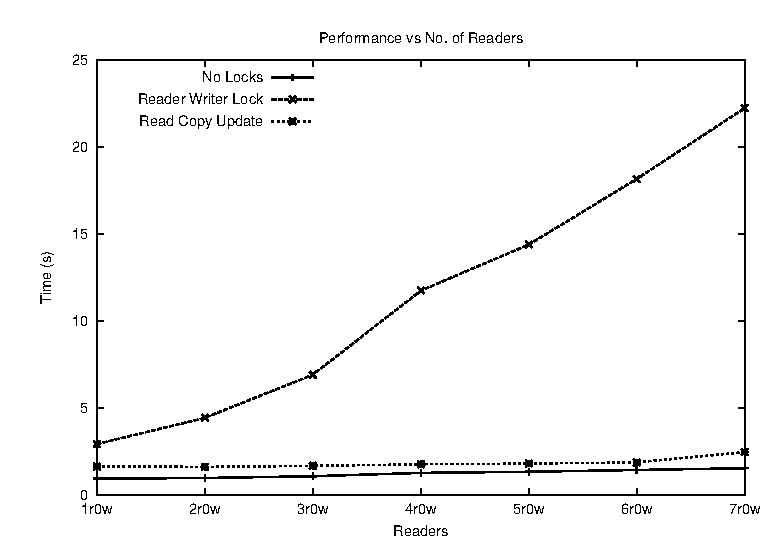
\includegraphics[scale = 0.7]{../images/graphs/macro_vr_0w}
\caption{Performance of increasing number of readers with zero writers using the 167k routing table.}
\label{img:macro_vr_0w}
\end{figure}

\begin{figure}[tph]
\includegraphics[scale = 0.7]{../images/graphs/profile_locks_macro_rwl_vr_0w}
\caption{Percentage time spent in contending for the lock for a pure reader workload.}
\label{img:profile_rwl_locks_vr_0w}
\end{figure}

From Figure \ref{img:macro_vr_0w}, we see that RCU scales much better
than the reader-writer lock version. RCU is always within $2$ times
the vanilla version. Time taken by the reader-writer lock increases
linearly and is up to $22$ times slower than the version without
locks.

These results validate our claim that RCU is wait-free and lock-free
for readers. In the RCU version readers do not create any
synchronization overhead. Readers in the reader-writer lock version
update a shared lock variable before they access the routing
table. The state of the shared variable needs to be updated through
all cores. As the number of threads increases, the contention causes
cache line bouncing and increased usage of the processor bus
bandwidth. The amount of time spent in acquiring a lock to enter
the read side critical section shown in \ref{img:profile_rwl_locks_vr_0w}. The graph shows an increasing amount of time spent contending for the lock with an increase in the number of threads. We can therefore attribute the  linear increase in time as the number of readers increase to the lock contention. This data was obtained for the benchmark shown in Table \ref{tbl:macro_vr_0w} using the Dtrace profiler. 

\subsubsection{Read Intensive Workload With One Writer}
\begin{table}[tph]
\begin{center}
\begin{table}[tph]
\begin{center}
\begin{tabular}{|l|l|l|l|}
\hline Workload &Reader-Writer Lock (s) & RCU (s) \\
\hline  reader(s)cu & 2.915 & 1.610\\
\hline  reader(s)cu & 4.425 & 1.600\\
\hline  reader(s)cu & 6.900 & 1.660\\
\hline  reader(s)cu & 11.737 & 1.750\\
\hline  reader(s)cu & 14.387 & 1.790\\
\hline  reader(s)cu & 18.160 & 1.860\\
\hline  reader(s)cu & 22.242 & 2.450\\
\hline
\end{tabular}
\end{center}
\label{tbl:writeintensive}
\caption{Performance comparison over a pure reader workload}
\end{table}

\end{center}
\caption{Performance comparison of increasing number of readers and one writer with the 167k routing table.}
\label{tbl:macro_vr_1w}
\end{table}


\begin{figure}[tph]
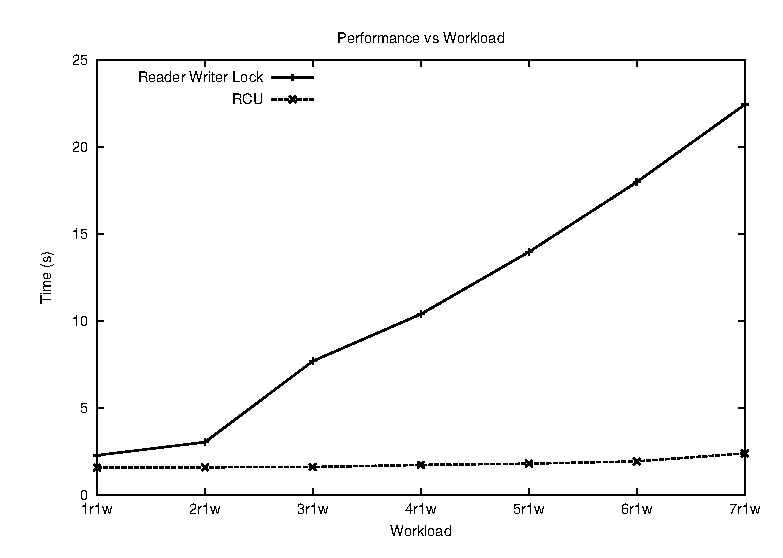
\includegraphics[scale = 0.7]{../images/graphs/macro_vr_1w}
\caption{Performance of increasing number of readers and one writer with the 167k routing table.}
\label{img:macro_vr_1w}
\end{figure}


\begin{figure}[tph]
\includegraphics[scale = 0.7]{../images/graphs/profile_locks_macro_rwl_vr_1w}
\caption{Percentage time spent in contending for the lock for a workload with increasing number of readers and one writer.}
\label{img:profile_rwl_locks_vr_1w}
\end{figure}

We also conducted a benchmark which consisted of one updater and an
increasing number of readers. The results are shown in Figure
\ref{img:macro_vr_1w} and Table \ref{tbl:macro_vr_1w}.

We see from Figure \ref{img:macro_vr_1w} that RCU scales far better
than the reader-writer lock. Time taken by the reader-writer lock
increases linearly with the number of threads. The reader-writer lock
version is over nine times slower than the RCU version for the
workload consisting of 7 readers and 1 writer. Figure \ref{img:profile_rwl_locks_vr_1w} shows the percentage time spent in contending for the lock to enter the read side critical section. We can attribute the linear increase in time to the increasing lock contention. RCU does not acquire any locks in this workload. We can clearly see that RCU
outperforms the reader-writer lock for a read intensive workload with some writers.

\subsubsection{Write Intensive Workloads}
We have seen that RCU outperforms the Reader-Writer lock for reader heavy workloads. For completeness, we look at some workloads which are not common for a router: writer heavy workloads. The performance of a workload with zero readers and increasing number of writers is shown in  Figure \ref{img:macro_0r_vw} and Table \ref{tbl:macro_0r_vw}. Here, we see that the Reader-Writer Lock outperforms RCU by a factor of . We attribute this to the increased memory footprint and increased overhead in management of the reclaim lists. **Justify.

The performance of a workload consisting of one reader and increasing number of writers is shown in  Figure \ref{img:macro_1r_vw} and Table \ref{tbl:macro_1r_vw}. Although RCU does not scale, we see that it performs better than the Reader-Writer Lock.

It is clear that RCU is not as fabulous for write intensive workloads. These workloads are very uncommon for a typical router and we can accept this behavior.
 
\begin{table}[tph]
\begin{center}
\begin{tabular}{|l|l|l|l|l|}
\hline Workload &Reader-Writer Lock (s) & RCU (s) & $\frac{\mbox{Reader-Writer Lock}}{\mbox{RCU}} $ \\
\hline 0 readers 1 writer & 0.180 & 0.182&0.986\\
\hline 0 readers 2 writers & 0.203 & 0.225&0.900\\
\hline 0 readers 3 writers & 0.230 & 0.295&0.780\\
\hline 0 readers 4 writers & 0.258 & 0.362&0.710\\
\hline 0 readers 5 writers & 0.307 & 0.435&0.707\\
\hline 0 readers 6 writers & 0.352 & 0.502&0.701\\
\hline 0 readers 7 writers & 0.407 & 0.588&0.694\\
\hline 0 readers 8 writers & 0.453 & 0.660&0.686\\
\hline
\end{tabular}

\end{center}
\caption{Performance comparison of increasing number of writers and zero readers using the 167k routing table.}
\label{tbl:macro_0r_vw}
\end{table}


\begin{figure}[tph]
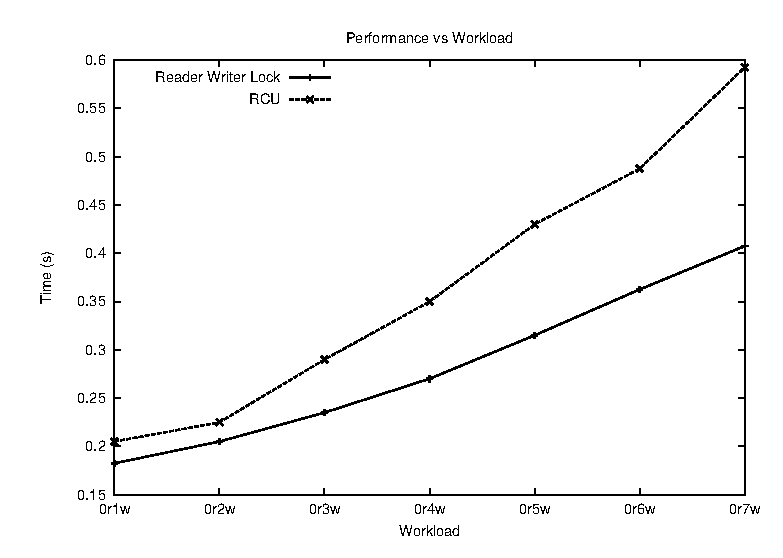
\includegraphics[scale = 0.7]{../images/graphs/macro_0r_vw}
\caption{Performance of increasing number of writers and zero readers with the 167k routing table.}
\label{img:macro_0r_vw}
\end{figure}


\begin{table}[tph]
\begin{center}
\begin{tabular}{|l|l|l|l|l|}
\hline Workload &Reader-Writer Lock (s) & RCU (s) & $\frac{\mbox{Reader-Writer Lock}}{\mbox{RCU}} $ \\
\hline 1 reader 1 writer & 2.260 & 1.540&1.468\\
\hline 1 reader 2 writers & 2.335 & 1.593&1.466\\
\hline 1 reader 3 writers & 2.397 & 1.677&1.429\\
\hline 1 reader 4 writers & 2.467 & 1.962&1.257\\
\hline 1 reader 5 writers & 2.547 & 2.078&1.226\\
\hline 1 reader 6 writers & 2.605 & 2.408&1.082\\
\hline 1 reader 7 writers & 2.663 & 2.310&1.153\\
\hline
\end{tabular}

\end{center}
\caption{Performance comparison of increasing number of writers and one reader using the 167k routing table.}
\label{tbl:macro_1r_vw}
\end{table}


\begin{figure}[tph]
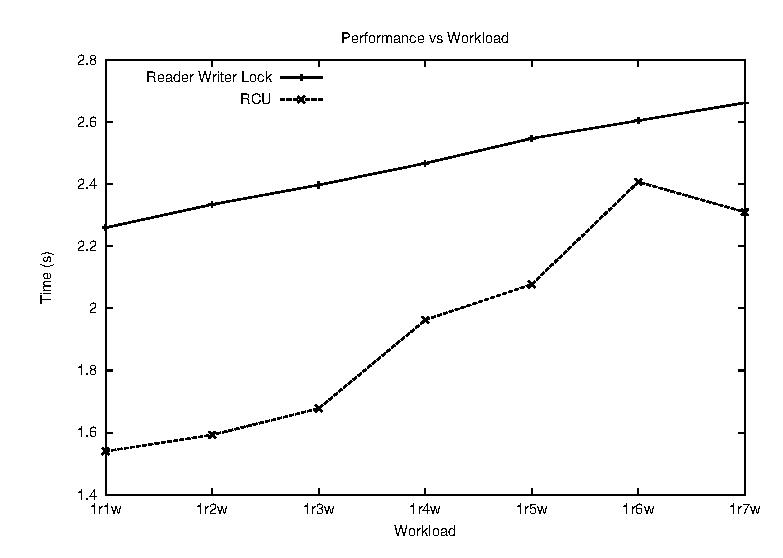
\includegraphics[scale = 0.7]{../images/graphs/macro_1r_vw}
\caption{Performance of increasing number of writers and one reader with the 167k routing table.}
\label{img:macro_1r_vw}
\end{figure}

\subsection{Micro-benchmarks}
\label{sec:microbenchmarks}
The micro-benchmarks have tests which repeatedly access a small set of addresses in a very short time span.
As with macro-benchmarks, we are interested mainly in read heavy workloads. We look at write heavy workloads for completeness.

\paragraph{Pure Reader Workload}
Here we consider a workload consisting of only readers. We look at how the reader-writer lock and RCU perform against the unmodified vanilla version.
As we can see from Table \ref{tbl:micro_vr_0w} which is represented in Figure \ref{img:micro_vr_0w}, the reader-writer lock is up to 50 times slower than a version without locks.
The reader-writer lock does not scale with an increase in the number of threads. The RCU version scales with an increase in the number of threads. The RCU version is also within 1.5 times the performance of the version without any locks.

The Reader-Writer lock spends time acquiring a lock on reads while RCU does not have any additional overhead for readers. Any additional overhead of RCU over the vanilla version is due to the overhead in checking reclaim lists and detecting quiescent states.

The Click configuration file used for this purpose is shown in Listing \ref{lst:readercomparison}.
\begin{table}
\begin{center}
\input{micro_vr_0w.tex}
\end{center}
\label{tbl:micro_vr_0w}
\caption{Performance comparison over a workload with increasing number of readers and zero writers.}
\end{table}

\begin{figure}[tph]
\fbox{
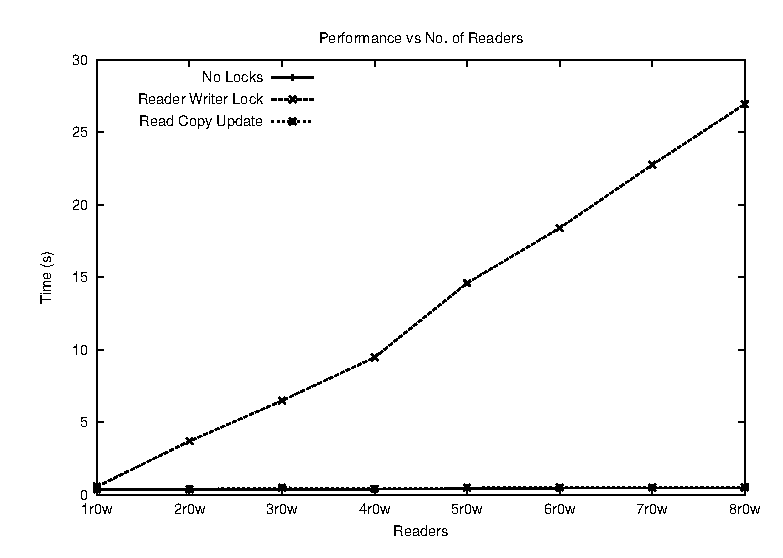
\includegraphics[scale = 0.7]{../images/graphs/micro_vr_0w}
}
\caption{Performance comparison over a workload with increasing number of readers and zero writers.}
\label{img:micro_vr_0w}
\end{figure}

\begin{lstlisting}[float=tph, caption = A Click configuration file for 4 readers, label =lst:readercomparison]
// 4 readers using the RCU (fine grained locking version)
// of RadixIPLookup.
Idle
 -> r :: RadixIPLookup106(
                1.1.1.0/32  8.1.1.1 0,
                0.0.0.0/0   8.1.1.1 0,
                ) 
 -> Idle;

reader :: ReadRadixIPLookup106(r);
reader1 :: ReadRadixIPLookup106(r);
reader2 :: ReadRadixIPLookup106(r);
reader3 :: ReadRadixIPLookup106(r);
StaticThreadSched(
        reader 0,
        reader1 1,
        reader2 2,
        reader3 3
);

DriverManager(stop);

\end{lstlisting}

\paragraph{Read Intensive workloads}
We now compare the performance of RCU over the reader-writer lock in the presence of a writer. This workload reflects typical router usage. We refer the reader to Table \ref{tbl:micro_vr_1w} and Figure \ref{img:micro_vr_1w} for the results.
RCU scales over an increase in the number of threads, however the reader-writer lock does not scale with an increase in the number of readers. This can be attributed to time spent waiting to acquire the lock before reading or writing in the Reader-Writer Lock version.

\begin{table}[tph]
\begin{center}
\input{micro_vr_1w.tex}
\end{center}
\label{tbl:micro_vr_1w}
\caption{Performance comparison of increasing number of readers with one writer.}
\end{table}

\begin{figure}[tph]
\begin{center}
\fbox{
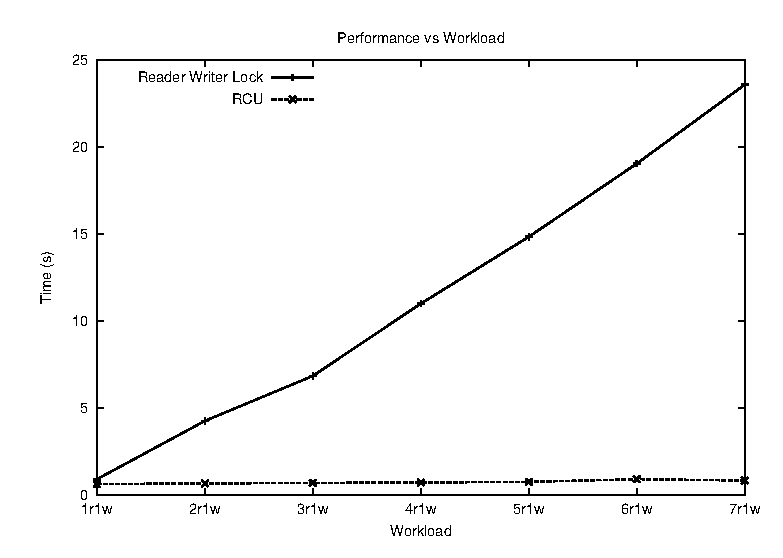
\includegraphics[scale = 0.7]{../images/graphs/micro_vr_1w}
}
\caption{Performance comparison of increasing number of readers with one writer.}
\label{img:micro_vr_1w}
\end{center}
\end{figure}

\paragraph{Write Intensive workloads}
We now compare the performance of RCU with the reader-writer lock for a write intensive workload. The performance of a workload with one reader and increasing number of writers is shown in Table \ref{tbl:micro_1r_vw} and Figure \ref{img:micro_1r_vw}. The performance of a workload with zero readers and increasing number of writers is shown in Table \ref{tbl:micro_0r_vw} and Figure \ref{img:micro_0r_vw}. In both cases, the reader-writer lock performs better than RCU. We attribute this to additional overhead caused due to lock contention to free stale data in quiescent states. When there are more writers, there is more stale data. Since these benchmarks target a very small set of routes, the reclamation also has contention for the same memory locations.

\begin{table}[tph]
\begin{center}
\input{micro_0r_vw.tex}
\end{center}
\label{tbl:micro_0r_vw}
\caption{Performance comparison of increasing number of writers with zero readers.}
\end{table}

\begin{figure}[tph]
\begin{center}
\fbox{
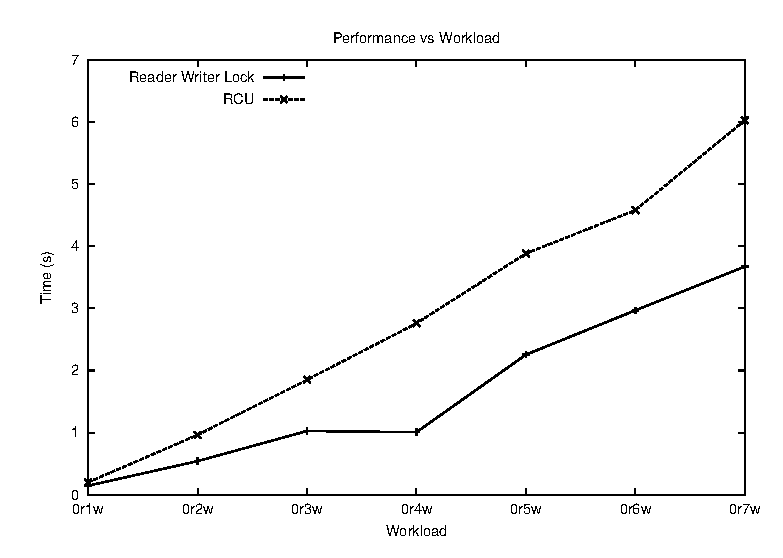
\includegraphics[scale = 0.7]{../images/graphs/micro_0r_vw}
}
\caption{Performance comparison of increasing number of writers with zero readers.}
\label{img:micro_0r_vw}
\end{center}
\end{figure}

\begin{table}[tph]
\begin{center}
\input{micro_1r_vw.tex}
\end{center}
\label{tbl:micro_1r_vw}
\caption{Performance comparison of increasing number of writers with one reader.}
\end{table}

\begin{figure}[tph]
\begin{center}
\fbox{
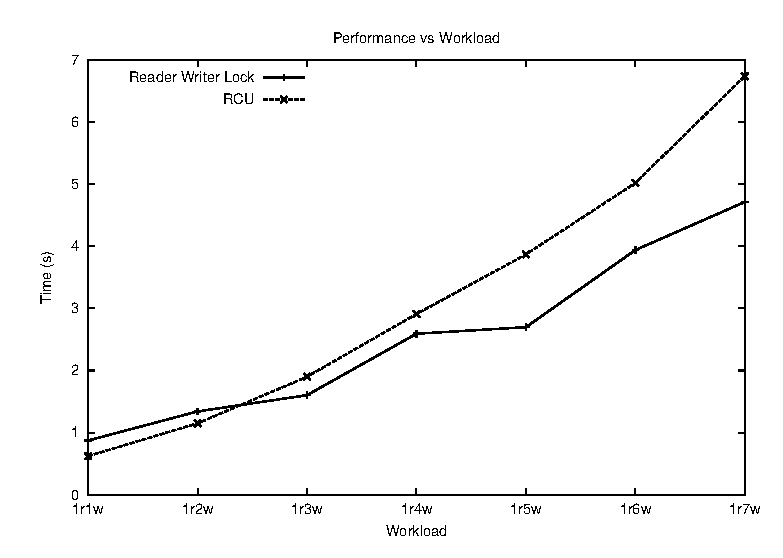
\includegraphics[scale = 0.7]{../images/graphs/micro_1r_vw}
}
\caption{Performance comparison of increasing number of writers with one reader.}
\label{img:micro_1r_vw}
\end{center}
\end{figure}


\section{Conclusion}
Lookup performance in a software router such as Click is crucially
important. Leveraging multicore processors which are available in almost all commodity hardware
today is a feasible way to improve performance. This document has outlined an efficient way to achieve a fast and safe multicore solution.


The primary challenges in implementing RCU for Click were to
identify quiescent states in a way which could be applied to all
elements. 

We have built an RCU framework for userlevel Click invlolving a
mechanism to detect quiescent states and an API which can be used by
a userlevel element in Click.

We have verified through our benchmarks that
this mechanism does indeed have a very low reader side overhead
(within two times the original version). The RCU approach is also up to
70\% better than a reader-writer lock on read intensive workloads.

\section{Future Work}

%\begin{enumerate}
%\item Implement RCU for RadixIPLookup if Radix nodes are deleted when a route is removed.
%\item Implement RCU for the Radix Tree: Currently, RCU has been only used on the vector. A coarse grained lock is acquired around updates to the Radix Tree.
%\end{enumerate}

Our approach uses RCU for the vector in RadixIPLookup, however a course grained lock is acquired for updates to the radix tree. The size of the radix tree depends on the size of the routing table, which is typically very large. Thus implementing RCU based synchronization for the radix tree would be very useful.
\section{Acknowledgements}
I am tremendously grateful to my advisor, Professor Eddie Kohler for his continued guidance, support and ideas.
Rohit Kumar contributed equally to this project. I am grateful to him for insightful discussions, code and comments.
\bibliography{rcu_report}
\bibliographystyle{plain}
\end{document}

